
\chapter{Methoden und Material}\label{method}

\section{Modulverarbeitung}\label{module}
\textbf{TODO, Anpassung der House-Brackmann Skala hier migirieren}

\begin{table}[!htb]\vspace{1ex}\centering
  \begin{tabular}{c||c|c|c|c|}
  Grad & Symmetrie    & Stirn  & Lidschluss    & Mund         \\ \hline\hline
  I    & Normal       & Normal & vollständig   & Normal       \\ \hline
  II  & Normal & Normal                                                        & vollständig & \begin{tabular}[c]{@{}c@{}}minimale\\ Asymmetrie\end{tabular} \\ \hline
  III & Normal & \begin{tabular}[c]{@{}c@{}}minimale\\ Asymmetrie\end{tabular} & vollständig & \begin{tabular}[c]{@{}c@{}}minimale\\ Asymmetrie\end{tabular} \\ \hline
  IV   & Normal       & keine  & unvollständig & Asymmetrisch \\ \hline
  V    & Asymmetrisch & keine  & unvollständig & Asymmetrisch \\ \hline
  VI   & keine        & keine  & unvollständig & keine        \\ \hline
  \end{tabular}
  \caption[Todo]{Todo}\label{cap:housebrackmannnew}
\vspace{2ex}\end{table}\label{table:housebrackmannnew}





\begin{figure}[h]
\begin{center}
\begin{tikzpicture}[->,>=stealth',shorten >=1pt,auto,node distance=2.5cm,semithick]
  \tikzstyle{every state}=[fill=cyan,draw=black,text=black]

  \tikzstyle{level1} = [rectangle, draw, fill=green!40!blue!20, text width=8cm, text centered, inner sep=1pt  , minimum height=2cm]
  \tikzstyle{level2} = [rectangle, draw, fill=blue!20,          text width=2cm, text centered, rounded corners, minimum height=3cm]
  \tikzstyle{level3} = [rectangle, draw, fill=green!40!blue!20, text width=8cm, text centered, inner sep=1pt  , minimum height=2cm]
  \tikzstyle{level4} = [rectangle, draw=white, fill=white, text width=1cm, text centered, minimum height=0.1cm, minimum width=0.1cm]

  \tikzstyle{container} = [draw, rectangle, dashed, inner sep=8pt, minimum width=15cm]

  \node[level4]         (Z1)                                 {};

  \node[level1]         (A) [left of=Z1, xshift=8cm]        {Regions of Interest};
  \node[level2]         (B) [below left  of=A, yshift=-2cm] {Lidschluss};
  \node[level2]         (C) [below right of=A, yshift=-2cm] {Mund};
  \node[level2]         (D) [left  of=B]                    {Symmetrie};
  \node[level2]         (E) [right of=C]                    {Stirn};
  \node[level3]         (F) [below right of=B, yshift=-2cm] {Automat};
  \node[container, fit=(B) (C) (D) (E)] (his) {};
    \node at (his.north west) [below right,node distance=0 and 0] {Module};

  \node[level4]         (Z2) [right of=F, xshift=3cm]        {};

  \path (Z1) edge [out=0   , in=180] node [left, xshift=-0.3cm]                {Input} (A)

        (A) edge [out=-145, in=90 ] node [right, yshift=-0.1cm, xshift=0cm   ] {$x_{lidschluss}$} (B) %Lidschluss
            edge [out=-35 , in=90 ] node [left , yshift=-0.1cm, xshift=0cm   ] {$x_{mund}$} (C) %Mund
            edge [out=-160, in=90 ] node [above, yshift=-0.5cm, xshift=0.8cm ] {$x_{symmetrie}$} (D) %Symmetrie
            edge [out=-20 , in=90 ] node [above, yshift=-0.5cm, xshift=-0.5cm] {$x_{stirn}$} (E) %Stirn
        (B) edge [out=-90 , in=145] node [right, yshift=0.1cm , xshift=0cm   ] {$y_{lidschluss}$} (F)
        (C) edge [out=-90 , in=35 ] node [left , yshift=0.1cm , xshift=0cm   ] {$y_{mund}$} (F)
        (D) edge [out=-90 , in=160] node [below, yshift=0.5cm , xshift=0.8cm ]  {$y_{symmetrie}$} (F)
        (E) edge [out=-90 , in=20 ] node [below, yshift=0.5cm , xshift=-0.5cm]  {$y_{stirn}$} (F)

        (F) edge [out=0   , in=180] node [right, xshift=0.3cm]                {Output} (Z2);

\end{tikzpicture}
\caption[Darstellung der Modulbauweise]{{Schematische Darstellung der Module}\label{cap:module}}
\end{center}
\end{figure}\label{fig:module}

\clearpage
\section{Datensatz}\label{dataset}

\subsection{? 9 Bilder pro Patient / Concartenation}\label{cutting}
\textbf{TODO}

\subsection{Erkennung des Gesichtes und die Zerschneidung}\label{cutting2}
\textbf{TODO}




\section{?? Trainingsphase der Neuronalen Netze}\label{training}
\textbf{TODO}





\section{Oversampling zum Klassenausgleich}\label{oversamplingmethod}
\textbf{TODO}

\section{Early Fusion und Late Fusion}\label{fusionmethod}
\textbf{TODO}









\section{Caching}\label{caching}
\textbf{TODO: Problem schildern}


Zwei mögliche Lösungsansätze wären \ac{lru} und eine stationäre externe Datenbank als, der als temporären Cache agiert.

\subsection{Least Recently Used Cache}\label{lrucache}
\ac{lru}, bedetuet, der am längsten nicht zugegriffenen Eintrag wird aus dem Cache entfernt. Vergleichen lässt sich das mit einer Warteschlange mit begrenztem Platzinhalt. Aufgerufene Elemente reihen sich am Ende der Warteschlange ein (im dargestellten Array die linke Seite). Alle nachfolgenden wandern um eine Position nach vorne. Der Vorderste in der Warteschlange wird entfernt (Abb. \ref{cap:lrucache}), sobald ein noch nicht bekannes Element einreiht. Dieses neue Element muss zur Laufzeit initial berechnet werden. Danach ist es solange Verfügbar bis es wieder herausgeschoben wurde.

Einträge im Cache haben einen Index. Über diesen werden auf die dahinter liegenden Elemente zugegriffen. Sei $l$ die Länge des Caches und $\Sigma$ Indizes (z.B. A-Z). Insgesammt $l$ Elemente können im Cache für das schnelle Aufrufen vorgehalten werden.

\begin{figure}[h]
\begin{center}
\begin{tikzpicture}[->,>=stealth',shorten >=1pt,auto,node distance=4cm,semithick]

  \tikzstyle{style} = [rectangle, draw, fill=green!40!blue!20, text centered, inner sep=1pt  , minimum height=2cm, align=center]

  \node[style] (A)              {Cache\\ {[A,B,C,D,E]}};
  \node[style] (B) [right of=A] {Cache\\ {[\textbf{B},A,C,D,E]}};
  \node[style] (C) [right of=B] {Cache\\ {[\textbf{E},B,A,C,D]}};
  \node[style] (D) [right of=C] {Cache\\ {[\textbf{Z},E,B,A,C]}};

  \path (A) edge  node [yshift=-1cm, align=center] {B\\ \\ \textcolor{green}{Hit}} (B)
        (B) edge  node [yshift=-1cm, align=center] {E\\ \\ \textcolor{green}{Hit}} (C)
        (C) edge  node [yshift=-1cm, align=center] {Z\\ \\ \textcolor{red}{Miss}}  (D);

\end{tikzpicture}
\caption[Beispiel des \ac{lru}]{Beispiel des \ac{lru} mit $l=5$ und dem $\Sigma=A-Z$}\label{cap:lrucache}
\end{center}
\end{figure}\label{fig:lrucache}


Im Cache liegenden Elemente besizen eine kürzere Aufrufdauer als diejenigen, die nicht im Cache sind. Die \ac{wcet}, die Zeit welche benötigt wird um ein Element aufzufen, beträgt für

\begin{itemize}
\item im Cache liegende Elemente: $WCET_{ges}=WCET_{cache}$
\item nicht im Cache liegende Elemente: $WCET_{ges}=WCET_{cache} + WCET_{berechnung}$
\end{itemize}

Dabei ist $WCET_{cache}$ die Laufzeit, die für das Nachschauen der Elemente im Cache benötigt wird und $WCET_{berechnung}$ für die initiale Berechnung des abzuspeichernden Elementes beträgt. Solange $l$ nicht wesentlich kleiner als die Anzahl von Elementem im Dataloader ist, können teilweise Einträge wiederverwertet werden, wenn ein neuer Epoch in der Trainingsphase der Neuronalen Netze beginnt. Die Berechnung der recycelten Elemente kann so eingespart werden, woraus eine kürzere Laufzeit zu erwarten ist.






\subsection{Datenbank}\label{database}
Eine weitere Möglichkeit ist es, Elemente in eine relationale Datenbank zu speichern. Der Aufbau ist dabei relativ Identisch zu dem \ac{lru}. Über einen Index wird auf das benötigte Element zugegriffen, jedoch sind \textbf{alle} Elemente in der Datenbank gespeichert. Die \ac{wcet} beträgt immer die Zeit, welche zum Zugriff auf die Datenbank benötigt wird. Zusätzlich kommt die Rechenzeit hinzu, welche benötigt wird, um alle Elemente in die Datenbank einzutragen. Solange nicht auf den selben Index geschrieben wird, ist es ratsam die Einträge parallel in die Datenbank zu schreiben, um Rechenzeit zu sparen. Indexe müssen als Primärschlüssel einendeutig sein, damit keine Konflikte beim Schreiben und Lesen auftreten!

\begin{table}[h]\vspace{1ex}\centering
  \begin{tabular*}{9cm}{c|c}
  \textbf{Indizes (Primärschlüssel)} & \textbf{Elemente}
  \\\hline
  A   &  Bild 1 \\
  B   &  Bild 2 \\
  C   &  Bild 3 \\
  D   &  Bild 4 \\
  E   &  Bild 5 \\
  ... & ...

  \\\hline
  \end{tabular*}
  \caption[Beispieltabelle in einer relationalen Datenbank]{Beispieltabelle in einer relationalen Datenbank}\label{cap:database}
\vspace{2ex}\end{table}\label{table:database}


Vorteil dieser Methode ist es, die kurze Lesezeit von der Datenbank ($WCET_{read}$) auszunutzen, da diese kleiner ist als die Berechnung zur Laufzeit ($WCET_{berechnung}$). In der Trainingsphase werden $z$ Epochs durchlaufen. Dadurch werden statt  $WCET_{berechnung} * z$ nur $WCET_{read} * z$ Zeiteinheiten benötigt, wobei gilt $WCET_{berechnung} > WCET_{read}$. Dadurch kann die Trainingsphase schneller beendet werden.
































%\section{?Use Cases}\label{usecase}
% \paragraph{Definition:}
% Use Case Diagramme auch bekannt als „Anwendungsfalldiagramm“ werden verwendet, um das Verhalten des Systems aus Sicht der Benuter zu modellieren.
% Benuter (dargestellt als Strichmännchen) oder Systeme sind Akterue, die miteinander agieren, die den jeweiligen \Acp{uc} abbilden. Die jeweiligen Relationen zwischen Akteure und den \ac{uc} werden mit Linien verbunden. Möglich sind auch Verbingung zwischen \ac{uc}. Dabei können sie andere \ac{uc} optional Erweitern (extend) oder Inkludieren einen weiteren, der den Basis Use Case erweitert. Auch sind Generalisierungen (Vererbung) möglich. So werden alle Eigenschaften und Fälle auf die Spezialisierung übernommen. \textbf{TODO Quelle!!!}
%
%
% \paragraph{Use Cases des Experimentes (siehe Abb. \ref{cap:usecase}):}
% Nach Erfolgrecher Beendigung des Experimentes können die Anwendungsfälle definiert werden. Folgende Akterure kristallisieren sich aus den \ac{uc} heraus:
% \begin{itemize}
% \item Benutzer*innen (Benutzer*innen/Patient*innen, die eine Kategorisierung erwünscht)
% \item Administrator*innen (Verwalter des Systems)
% \item Docker Container (Instanz auf einem Server, der den Sourcecode laufen lässt und über eine Schnittstelle den Zugriff ernöglicht)
% \end{itemize}
%
% \begin{figure}[h]
% \begin{center}
%  \includesvg[width=0.98\textwidth]{./images/UseCase}
% \caption[Use Case Diagramm]{Anwendungsfälle des Experimentes als Use Cases beschrieben.}\label{cap:usecase}
% \end{center}
% \end{figure}\label{fig:usecase}
%
% Administrator*innen verwalten im allgemeinen das System. Diese führen die Trainingsphase aus und versuchen, so genau wie möglich, die Ergebnisse für den Hosue-Brackmann Grad, zu ermitteln. Dabei handelt sich es um ein Optimierungsproblem. Parameter können die Lernrate der Neuronalen Netze beeinfulssen. Auch welches Neuronale Netz zur Anwendung kommt wird von ihnen beeinflusst.
%
% Über einen API Zugriff können so Benutzer*innen für sich selbst die Detection starten indem sie über einen Request an den Server, der die Komponenten hostet, stellt. Dieser sendet ihnen nach der Berechnung das Ergebnis zurück. Im Hintergrund führt der Server, in dem Fall dargestellt als Docker-Container, der über eine IP-Adresse für die Aussenwelt erreichbar ist, die Berechnung aus.
%
%
% \begin{figure}[h]
% \begin{center}
%  \includesvg[width=0.98\textwidth]{./images/API_Request}
% \caption[Aktivitätsdiagramm eines schematischen Ablaufes eines  Requestes]{Aktivitätsdiagramm eines schematischen Ablaufes eines Requestes.}\label{cap:apirequest}
% \end{center}
% \end{figure}\label{fig:apirequest}



\section{Material}\label{module}
\textbf{TODO Datensatz erklären}


\begin{enumerate}
  \setlength\itemsep{-0.5em}
\item Ruhender Gesichtsausdruck
\item Augenbrauen heben
\item Lächeln, geschlossener Mund
\item Lächeln, geöffneter Mund
\item Lippen schürzen, \glqq Duckface\grqq{}
\item Augenschluss, leicht
\item Augenschluss, forciert
\item Nase rümpfen
\item Depression Unterlippe
\end{enumerate}



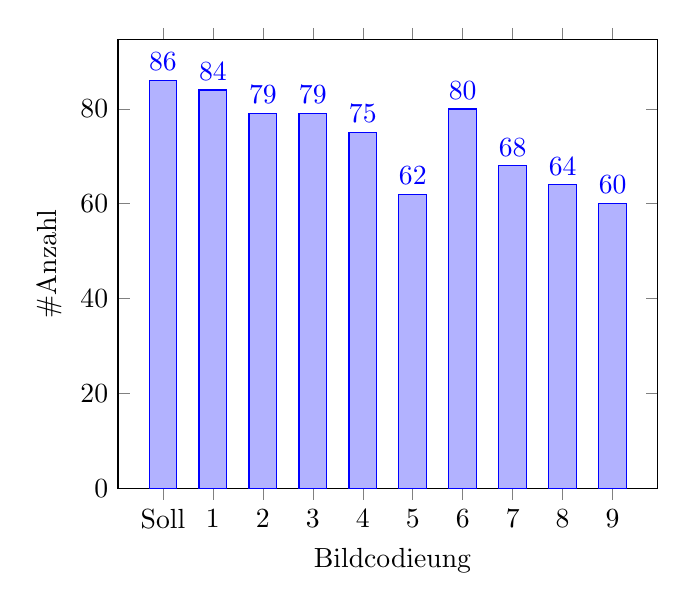
\begin{tikzpicture}
\begin{axis}
[
    ybar,
    ymin=0,
    %enlargelimits=0.15,
    ylabel={\#Anzahl}, % the ylabel must precede a # symbol.
    xlabel={\ Bildcodieung},
    symbolic x coords={Soll, 1, 2, 3, 4, 5, 6, 7, 8, 9},
    xtick=data,
    nodes near coords, % this command is used to mention the y-axis points on the top of the particular bar.
    nodes near coords align={vertical},
    ]
\addplot coordinates {(Soll,86) (1,84) (2,79) (3,79) (4,75)
                      (5,62)    (6,80) (7,68) (8,64) (9,60) };

\end{axis}
\end{tikzpicture}
